\begin{exercise}
      {ID-3cafc2ad6d4e3c35f1b5321aa27fa7e610df34fc}
      {Umfang}
  \ifproblem\problem\par
    Stelle einen Term zur Berechnung des Umfangs auf, und vereinfache ihn so weit wie möglich.
    \begin{center}
      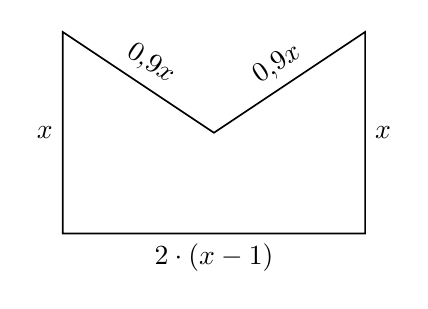
\begin{tikzpicture}[scale=0.64, line width=0.6]
        \draw (0, 0) -- (6, 0) -- (6, 4) -- (3, 2) -- (0, 4) -- cycle;
        \node[left]  at (0, 2) {$x$};
        \node[right] at (6, 2) {$x$};
        \node[below] at (3, 0) {$2\cdot(x-1)$};
        \path (6, 4) -- node[above, rotate=33.69] {$0,\!9x$} (3, 2);
        \path (3, 2) -- node[above, rotate=-33.69] {$0,\!9x$} (0, 4);
      \end{tikzpicture}
    \end{center}
  \fi
  %\ifoutline\outline\par
  %\fi
  %\ifoutcome\outcome\par
  %\fi
\end{exercise}
